\newpage
\chapter{METODE PENELITIAN} \label{Bab III}
% \isi{...} = bagian yang masih harus Anda lengkapi (tampil tebal dalam kurung siku).
\providecommand{\isi}[1]{\textbf{[#1]}}

\section{Alur Penelitian}
Penelitian ini terdiri atas tujuh tahap, yaitu identifikasi masalah dan studi literatur, pengumpulan data, analisis kebutuhan, pengembangan prototipe, pengujian, analisis hasil, serta kesimpulan dan saran. Tahap pengembangan prototipe diulang apabila prototipe belum sesuai kebutuhan sekolah. Alur penelitian ditunjukkan pada Gambar~\ref{fig:alur_penelitian}.

\begin{figure}[H]
    \centering
    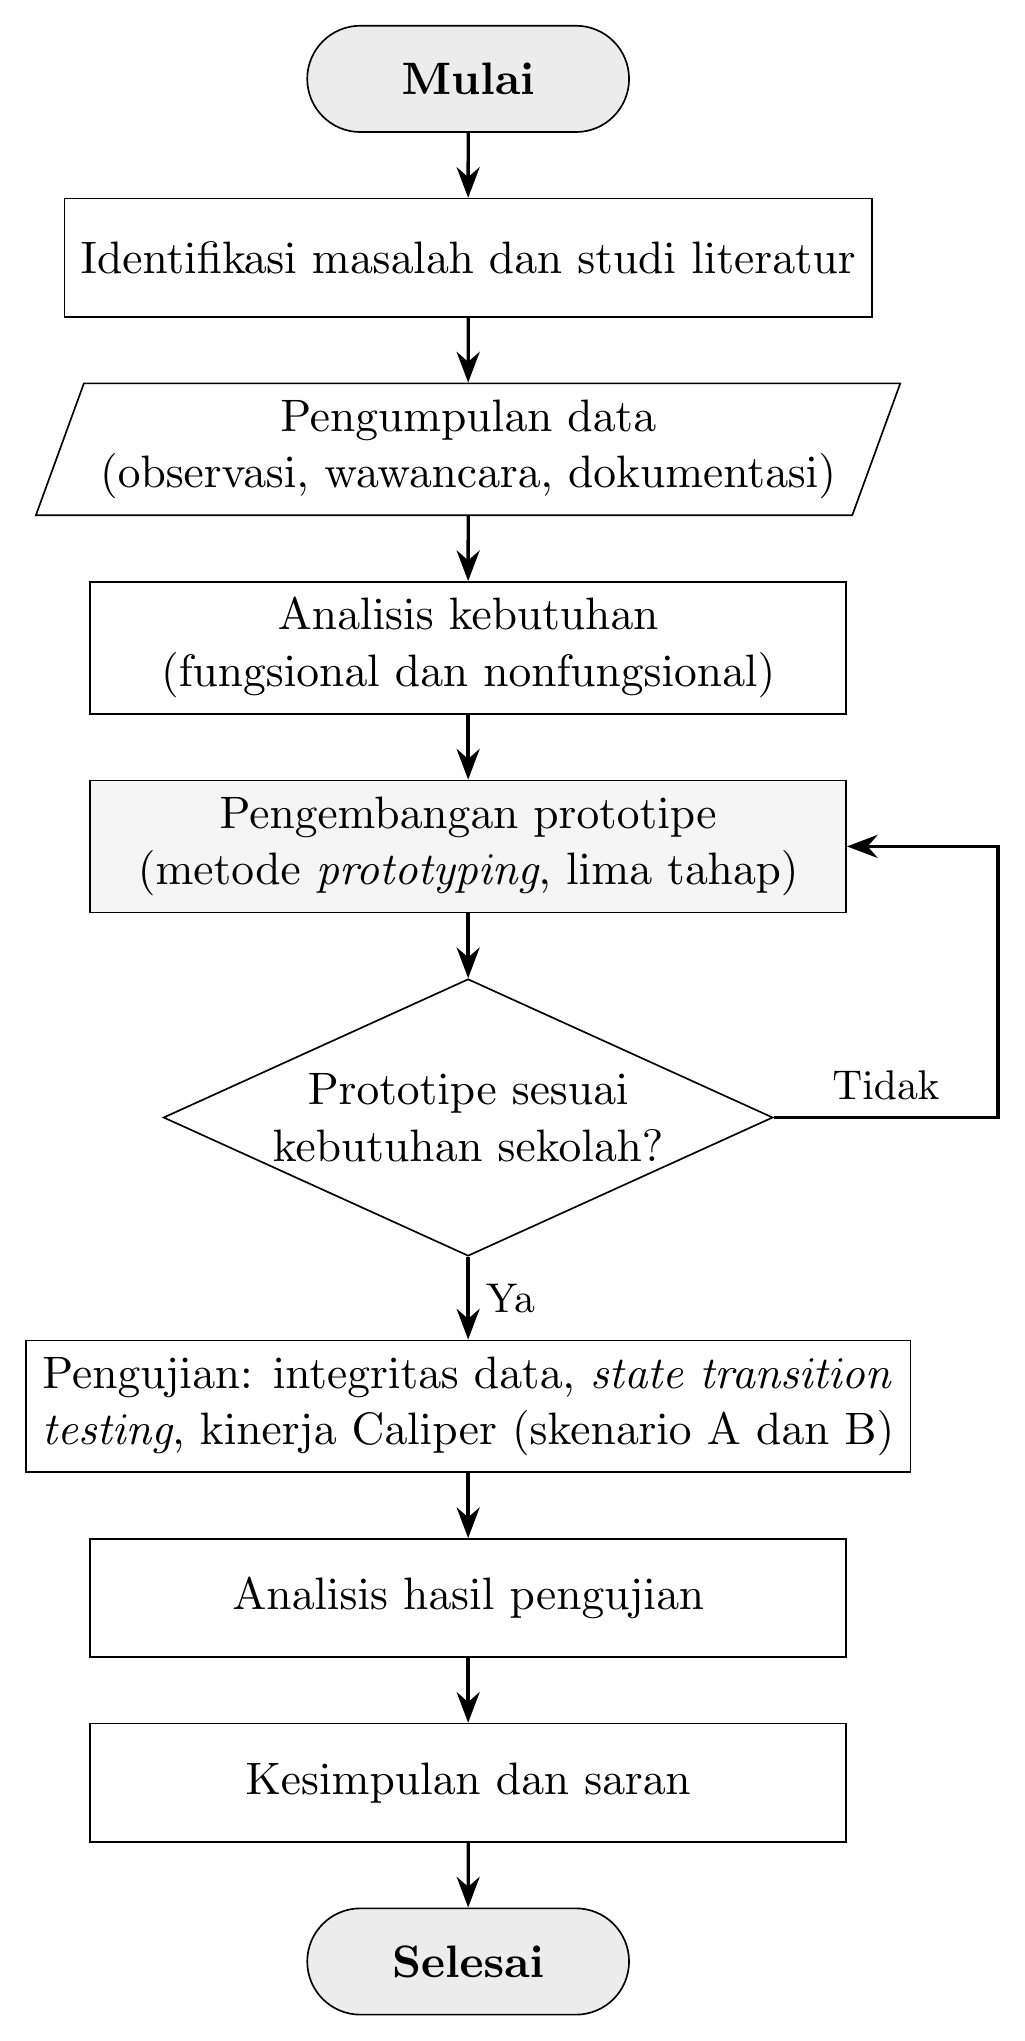
\includegraphics[width=0.45\textwidth]{figure/AlurPenelitian.png}
    \caption{Alur Penelitian}
    \label{fig:alur_penelitian}
\end{figure}

\section{Penjabaran Langkah Penelitian}
Setiap tahap pada Gambar~\ref{fig:alur_penelitian} dijabarkan pada subbab berikut. Tahap pengembangan prototipe mengikuti metode \textit{prototyping} yang dijelaskan lebih rinci pada Subbab~\ref{III.Metode}.

\subsection{Identifikasi Masalah dan Studi Literatur}
Tahap ini mengidentifikasi permasalahan penerbitan dan verifikasi SKL di SMAN 1 Gadingrejo, yaitu verifikasi manual melalui arsip fisik, arsip tanpa cadangan, kesalahan input data, dan kasus pemalsuan SKL. Studi literatur dilakukan terhadap lima penelitian utama dan dokumentasi resmi Hyperledger Fabric untuk menentukan celah penelitian dan teknologi yang digunakan, sebagaimana diuraikan pada Bab II. Dokumentasi kegiatan identifikasi masalah di SMAN 1 Gadingrejo ditunjukkan pada Gambar~\ref{fig:identifikasi_masalah}.

\begin{figure}[H]
    \centering
    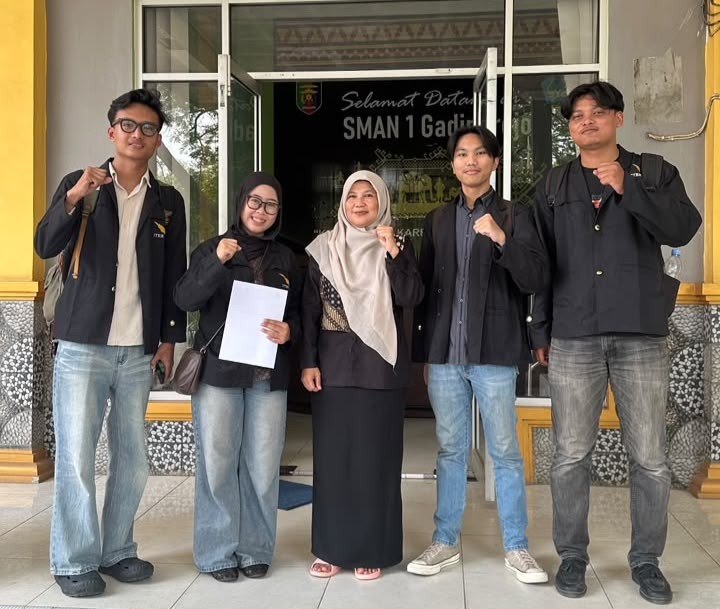
\includegraphics[width=0.7\textwidth]{figure/IdentifikasiMasalah.jpeg}
    \caption{Dokumentasi identifikasi masalah di SMAN 1 Gadingrejo}
    \label{fig:identifikasi_masalah}
    \vspace{2pt}
    {\footnotesize Sumber: dokumentasi peneliti (2026)}
\end{figure}

\subsection{Pengumpulan Data}
Data dikumpulkan melalui observasi, wawancara, dan dokumentasi di SMAN 1 Gadingrejo. Hasilnya berupa alur penerbitan SKL, peran dan kewenangan setiap pihak, format SKL, serta data siswa yang lulus pada tahun 2026 yang digunakan atas izin sekolah. Rincian cara pengumpulan data dijelaskan pada Subbab~\ref{III.Metode}. Dokumentasi kegiatan pengumpulan data di SMAN 1 Gadingrejo ditunjukkan pada Gambar~\ref{fig:pengumpulan_data}.

\begin{figure}[H]
    \centering
    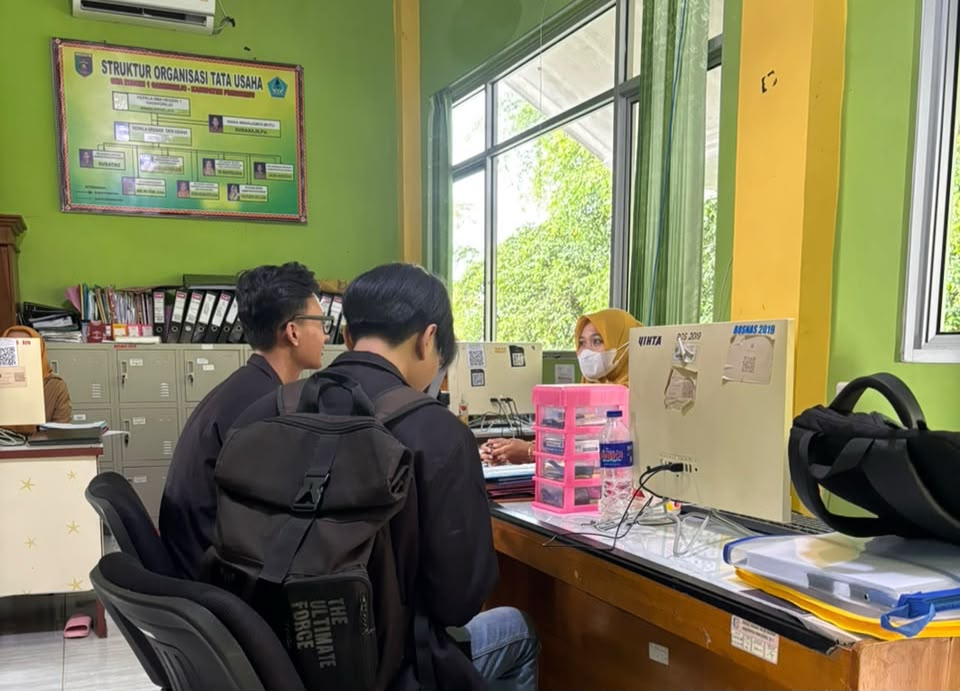
\includegraphics[width=0.7\textwidth]{figure/PengumpulanData.jpeg}
    \caption{Dokumentasi pengumpulan data di SMAN 1 Gadingrejo}
    \label{fig:pengumpulan_data}
    \vspace{2pt}
    {\footnotesize Sumber: dokumentasi peneliti (2026)}
\end{figure}

\subsection{Analisis Kebutuhan}
Tahap ini mengolah hasil observasi, wawancara, dan dokumentasi menjadi kebutuhan sistem. Analisis dimulai dengan mengidentifikasi pihak yang berinteraksi dengan sistem, yaitu staf tata usaha, kepala tata usaha, wakil kepala sekolah bidang kurikulum, kepala sekolah, dan pihak eksternal sebagai verifikator. Selanjutnya, setiap kendala yang ditemukan di sekolah dipetakan menjadi kebutuhan yang harus dipenuhi sistem, sedangkan isi minimal SKL mengikuti pedoman penerbitan SKL~\cite{Kepmendikdasmen2026SKL}.

Kebutuhan dibagi menjadi kebutuhan fungsional, yaitu fungsi yang harus dapat dijalankan sistem, dan kebutuhan nonfungsional, yaitu kualitas yang harus dipenuhi sistem. Hasil analisis kebutuhan ditunjukkan pada Tabel~\ref{table:3.kebutuhan}, dan setiap kebutuhan tersebut menjadi acuan dalam pengembangan prototipe dan penyusunan skenario pengujian.

\begin{table}[H]
    \centering
    \caption{Hasil analisis kebutuhan sistem}
    \label{table:3.kebutuhan}
    \footnotesize
    \renewcommand{\arraystretch}{1.25}
    \begin{tabular}{|>{\raggedright\arraybackslash}p{0.12\textwidth}|>{\raggedright\arraybackslash}p{0.48\textwidth}|>{\raggedright\arraybackslash}p{0.28\textwidth}|}
        \hline
        \textbf{Kode} & \textbf{Kebutuhan} & \textbf{Dasar kebutuhan} \\
        \hline
        \multicolumn{3}{|c|}{\textbf{Kebutuhan fungsional}} \\
        \hline
        KF-01 & Staf tata usaha dapat mengimpor data seluruh siswa satu angkatan dari satu berkas Excel/CSV, dan setiap baris divalidasi sebelum disimpan & Kesalahan input dan lamanya penyusunan SKL \\
        \hline
        KF-02 & Data nilai mendukung jumlah dan jenis mata pelajaran yang berbeda untuk setiap siswa, dan rata-rata dihitung otomatis & Mata pelajaran pilihan pada Kurikulum Merdeka \\
        \hline
        KF-03 & Draf SKL dapat diubah per siswa atau diimpor ulang sebelum diverifikasi kepala tata usaha & Koreksi data sebelum diperiksa \\
        \hline
        KF-04 & SKL hanya terbit setelah diverifikasi kepala tata usaha serta disetujui wakil kepala sekolah bidang kurikulum dan kepala sekolah secara berurutan; persetujuan dapat dilakukan sekaligus untuk banyak SKL, tetapi tetap tercatat per SKL & Alur kewenangan di sekolah dan jumlah sekitar 396 SKL \\
        \hline
        KF-05 & Wakil kepala sekolah bidang kurikulum dan kepala sekolah dapat menolak SKL disertai alasan & Koreksi sebelum terbit \\
        \hline
        KF-06 & Nomor surat SKL dibuat otomatis dan berurutan dari nomor awal yang ditetapkan sekolah & Penomoran surat yang dilakukan manual \\
        \hline
        KF-07 & SKL hanya dapat dicabut dengan persetujuan minimal dua dari tiga pejabat & Pencegahan pencabutan sepihak \\
        \hline
        KF-08 & Pihak eksternal dapat memeriksa keaslian, nomor surat, dan status SKL secara daring & Verifikasi manual melalui arsip fisik \\
        \hline
        \multicolumn{3}{|c|}{\textbf{Kebutuhan nonfungsional}} \\
        \hline
        KNF-01 & Perubahan isi SKL setelah dicatat dapat terdeteksi & Kasus pemalsuan SKL \\
        \hline
        KNF-02 & Data pribadi siswa tidak dapat dibaca pihak di luar sekolah & Pelindungan data pribadi~\cite{UU27Tahun2022} \\
        \hline
        KNF-03 & Catatan SKL tersimpan dalam lebih dari satu salinan & Arsip fisik tanpa cadangan \\
        \hline
        KNF-04 & Jaringan mampu mencatat sekitar 396 SKL per angkatan dengan \textit{success rate} mendekati 100\% & Jumlah lulusan per angkatan \\
        \hline
    \end{tabular}
\end{table}

\subsection{Pengembangan Prototipe}
Prototipe \textit{permissioned blockchain} dan \textit{smart contract} multi-otoritas dibangun dengan metode \textit{prototyping} yang terdiri atas lima tahap, yaitu \textit{communication}, \textit{quick plan}, \textit{modeling quick design}, \textit{construction of prototype}, serta \textit{deployment, delivery}, dan \textit{feedback}~\cite{Adim2025Prototype}. Masukan tahap ini adalah kebutuhan pada Tabel~\ref{table:3.kebutuhan}, sedangkan keluarannya berupa jaringan Hyperledger Fabric yang berjalan, \textit{chaincode} SKL yang menerapkan aturan multi-otoritas, serta konfigurasi \textit{private data collection} untuk data pribadi siswa.

Setiap putaran pengembangan diakhiri dengan demonstrasi prototipe kepada pihak sekolah. Prototipe dinyatakan sesuai apabila pihak sekolah menyatakan bahwa urutan persetujuan, aturan penolakan, dan aturan pencabutan yang dijalankan prototipe telah sesuai dengan prosedur penerbitan SKL di sekolah. Apabila belum sesuai, umpan balik dicatat dan prototipe diperbaiki pada putaran berikutnya. Rincian penerapan setiap tahap dijelaskan pada Subbab~\ref{III.Metode}.

\subsection{Pengujian}
Prototipe yang telah dinyatakan sesuai oleh pihak sekolah diuji dari tiga sisi untuk menjawab rumusan masalah kedua. Pengujian integritas data memeriksa apakah perubahan isi SKL dapat terdeteksi melalui ketidakcocokan nilai \textit{hash}. Pengujian kontrol akses dan alur persetujuan menggunakan \textit{black box testing} teknik \textit{state transition testing} untuk memeriksa apakah setiap peran hanya dapat menjalankan fungsi yang menjadi kewenangannya dan sesuai urutan. Pengujian kinerja menggunakan Hyperledger Caliper untuk mengukur \textit{throughput}, \textit{latency}, dan \textit{success rate}, termasuk perbandingan penerbitan oleh satu otoritas dan empat otoritas.

Pengujian fungsional dilakukan lebih dahulu karena pengujian kinerja hanya bermakna apabila aturan multi-otoritas sudah berjalan dengan benar. Seluruh pengujian dijalankan pada jaringan uji lokal di laptop peneliti. Rancangan skenario dan kasus uji dijelaskan pada Subbab~\ref{III.Pengujian}.

\subsection{Analisis Hasil}
Hasil pengujian diolah menggunakan rumus pada Bab II. Hasil pengujian integritas data dan \textit{state transition testing} dihitung sebagai persentase skenario yang sesuai harapan, sedangkan hasil pengujian Caliper diolah menjadi nilai rata-rata \textit{throughput}, \textit{latency}, dan \textit{success rate} dari tiga kali pengulangan untuk setiap laju kirim. Hasil skenario A dan B kemudian digunakan untuk menghitung \textit{overhead} multi-otoritas.

Hasil tersebut dianalisis dengan tiga cara. Pertama, hasil dibandingkan dengan hipotesis pada Subbab~\ref{III.Pengujian}. Kedua, hasil kinerja dibandingkan dengan hasil penelitian Dash dkk.~\cite{Dash2025Hyperledger} yang juga menggunakan Hyperledger Fabric dan Caliper. Ketiga, \textit{overhead} multi-otoritas dinilai terhadap kebutuhan sekolah, yaitu apakah tambahan waktu akibat persetujuan bertingkat masih wajar untuk menerbitkan sekitar 396 SKL per angkatan. Hasil analisis disajikan dalam bentuk tabel dan grafik pada Bab IV.

\subsection{Kesimpulan dan Saran}
Tahap terakhir adalah menarik kesimpulan berdasarkan hasil analisis. Kesimpulan disusun untuk menjawab kedua rumusan masalah, yaitu bagaimana \textit{permissioned blockchain} dan \textit{smart contract} multi-otoritas untuk SKL dirancang dan dibangun, serta bagaimana hasil pengujian integritas data, kontrol akses dan alur persetujuan, dan kinerja jaringannya.

Saran disusun berdasarkan keterbatasan yang ditemukan selama penelitian, misalnya kemungkinan pengembangan jaringan yang melibatkan lebih dari satu sekolah, penerapan pada dokumen akademik lain, atau penetapan masa retensi data pribadi siswa. Saran tersebut ditujukan bagi pihak sekolah dan peneliti selanjutnya.

\section{Alat dan Bahan}
\subsection{Alat}
Alat yang digunakan dalam penelitian ini adalah sebagai berikut.
\begin{enumerate}
    \item Laptop dengan spesifikasi sistem operasi \textit{Windows 11, processor AMD Ryzen 7 7730U (8 Core, 2,00 GHz), RAM 16 GB DDR4,} dan penyimpanan 512 GB.
    \item Sistem operasi Ubuntu 22.04 LTS, dijalankan melalui \textit{Windows Subsystem for Linux} 2 (WSL2) karena laptop menggunakan Windows.
    \item Docker Engine dan Docker Compose untuk menjalankan \textit{node} Fabric dalam bentuk kontainer.
    \item Hyperledger Fabric versi 2.5 dan Fabric CA versi 1.5.
    \item Bahasa pemrograman Go untuk membangun \textit{chaincode}, menggunakan pustaka \textit{fabric-contract-api-go} dan cid.
    \item Node.js versi 18 LTS dan Hyperledger Caliper versi 0.6.0 untuk pengujian kinerja.
    \item \textit{Code editor} Microsoft Visual Studio Code.
    \item Git dan GitHub untuk pengelolaan versi kode program.
\end{enumerate}

\subsection{Bahan}
Bahan yang digunakan dalam penelitian ini adalah sebagai berikut.
\begin{enumerate}
    \item Data siswa SMAN 1 Gadingrejo yang lulus pada tahun 2026, sekitar 396 siswa, yang diperoleh dan digunakan atas izin sekolah. Data hanya disimpan pada jaringan uji lokal, sedangkan contoh data yang ditampilkan dalam laporan menggunakan data samaran sesuai prinsip pelindungan data pribadi~\cite{UU27Tahun2022}.
    \item Format SKL SMAN 1 Gadingrejo serta hasil observasi dan wawancara dengan staf tata usaha, kepala tata usaha, wakil kepala sekolah bidang kurikulum, dan kepala sekolah.
    \item Keputusan Menteri Pendidikan Dasar dan Menengah Nomor 177 Tahun 2026 sebagai pedoman isi dan penerbitan SKL~\cite{Kepmendikdasmen2026SKL}.
    \item Dokumentasi resmi Hyperledger Fabric, Fabric CA, dan Hyperledger Caliper~\cite{FabricMSP,FabricCA,FabricPrivateData,Caliper}, serta artikel penelitian yang disitasi pada Bab II.
\end{enumerate}

\section{Metode Pengembangan} \label{III.Metode}
Subbab ini menjelaskan alur pengembangan, cara pengumpulan data, metode pengembangan, dan metode pengujian yang digunakan.

\subsection{Alur Pengembangan}
Pengembangan prototipe mengikuti metode \textit{prototyping}, yaitu prototipe dibangun secara cepat, diperlihatkan kepada pengguna, lalu diperbaiki berdasarkan umpan balik sampai sesuai kebutuhan~\cite{Adim2025Prototype}. Metode ini dipilih karena aturan kewenangan penerbitan SKL perlu dikonfirmasi langsung kepada pihak sekolah, dan rancangan seperti urutan persetujuan, aturan penolakan, dan pejabat yang berwenang mencabut SKL kemungkinan masih berubah setelah sekolah melihat prototipe. Alur pengembangan ditunjukkan pada Gambar~\ref{fig:alur_prototyping}.

\begin{figure}[H]
    \centering
    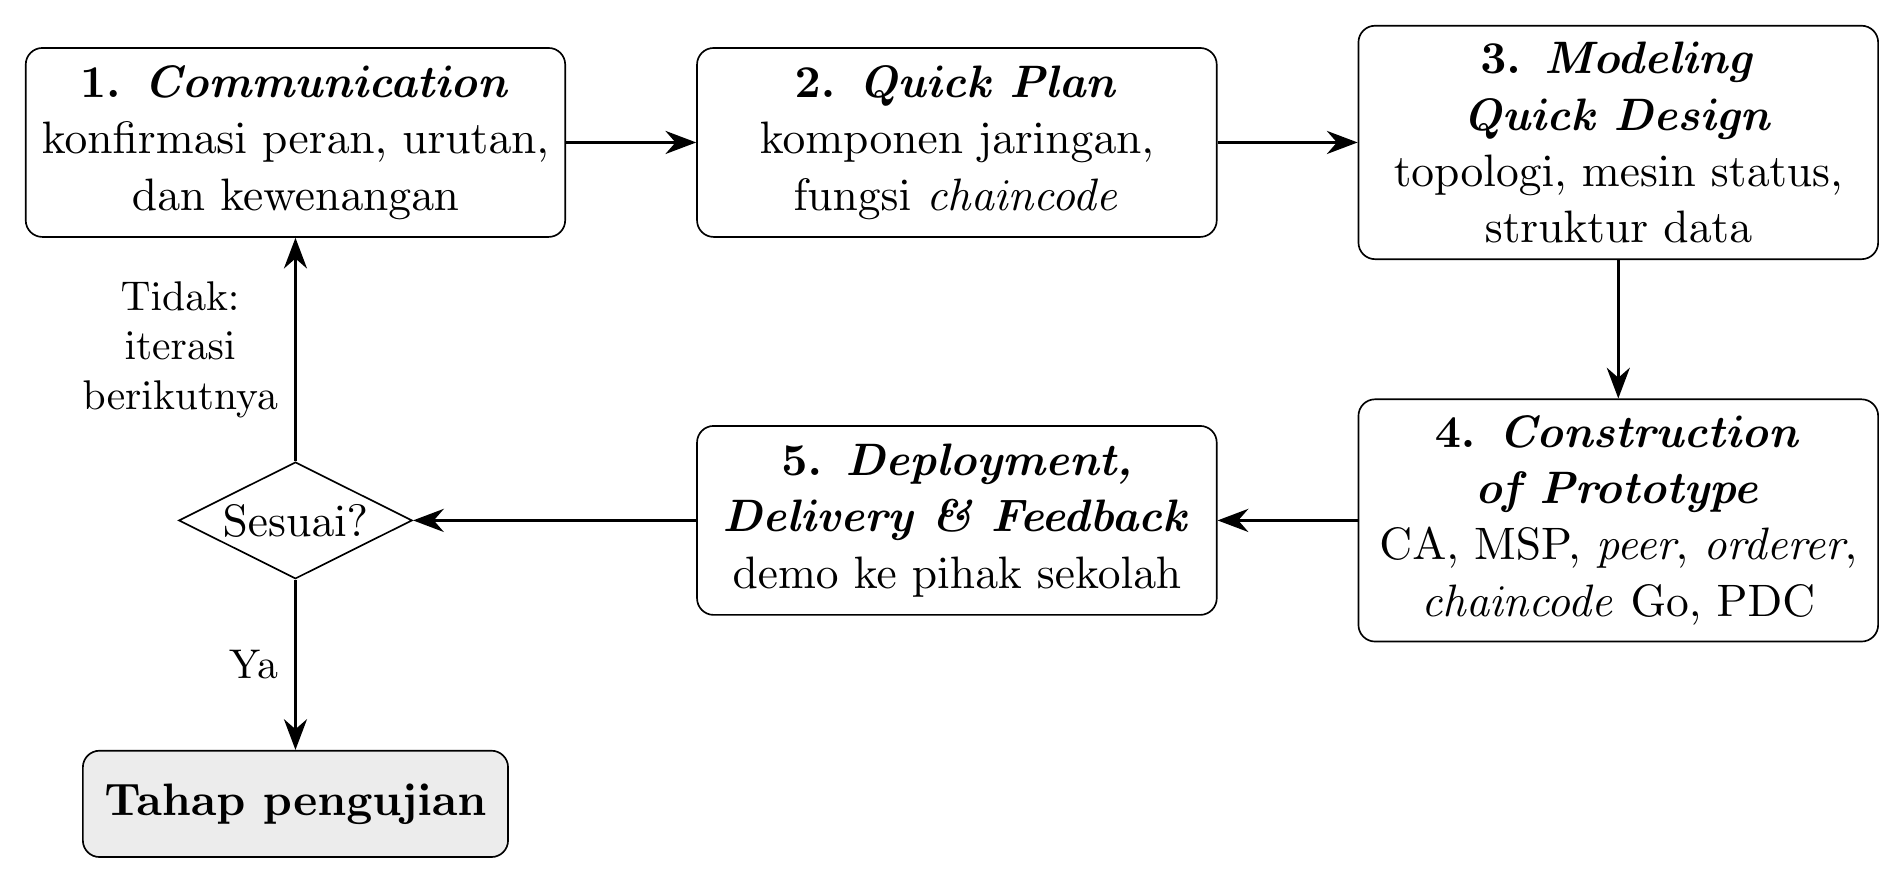
\includegraphics[width=0.95\textwidth]{figure/AlurPrototyping.png}
    \caption{Alur pengembangan dengan metode \textit{prototyping}}
    \label{fig:alur_prototyping}
    \vspace{2pt}
    {\footnotesize Sumber: diolah dari~\cite{Adim2025Prototype}}
\end{figure}

\subsection{Cara Pengumpulan Data}
Data dikumpulkan dengan tiga cara berikut.
\begin{enumerate}
    \item Observasi, dilakukan di ruang tata usaha SMAN 1 Gadingrejo pada 14 September dan 2 Oktober 2026 untuk mengamati proses penyusunan, pencetakan, pengarsipan, dan verifikasi SKL.
    \item Wawancara, dilakukan dengan kepala tata usaha, staf tata usaha, dan wakil kepala sekolah bidang kurikulum untuk mengetahui peran dan kewenangan setiap pihak, waktu penyusunan SKL, kendala yang dihadapi, dan kasus pemalsuan SKL.
    \item Dokumentasi, berupa format SKL dan data siswa yang lulus pada tahun 2026 yang diperoleh atas izin sekolah.
\end{enumerate}

\subsection{Metode Pengembangan Prototipe}
Kelima tahap metode \textit{prototyping}~\cite{Adim2025Prototype} diterapkan sebagai berikut.

\textbf{1. \textit{Communication}}

Peneliti mengonfirmasi kebutuhan kepada pihak sekolah, yaitu peran dan kewenangan staf tata usaha, kepala tata usaha, wakil kepala sekolah bidang kurikulum, dan kepala sekolah; urutan persetujuan; pejabat yang berwenang mencabut SKL; serta data yang wajib tercantum pada SKL, susunan kolom berkas leger nilai yang akan diimpor, dan format nomor surat SKL.

\textbf{2. \textit{Quick Plan}}

Peneliti menyusun rencana singkat yang berisi komponen jaringan, daftar fungsi \textit{chaincode}, struktur data, dan urutan pengerjaan. Jaringan terdiri atas satu organisasi karena SKL hanya diterbitkan dan disahkan secara internal oleh sekolah. \textit{Endorsement policy} mensyaratkan pengesahan dari dua \textit{peer} anggota SekolahMSP agar hasil eksekusi \textit{chaincode} pada satu \textit{peer} selalu dicocokkan dengan \textit{peer} lainnya. Rancangan komponen jaringan ditunjukkan pada Tabel~\ref{table:3.konfigurasi}.

\begin{table}[H]
    \centering
    \caption{Rancangan konfigurasi \textit{node} Hyperledger Fabric}
    \label{table:3.konfigurasi}
    \footnotesize
    \renewcommand{\arraystretch}{1.25}
    \begin{tabular}{|>{\raggedright\arraybackslash}p{0.25\textwidth}|>{\raggedright\arraybackslash}p{0.15\textwidth}|>{\raggedright\arraybackslash}p{0.48\textwidth}|}
        \hline
        \textbf{Komponen} & \textbf{Jumlah} & \textbf{Keterangan} \\
        \hline
        Organisasi (SekolahMSP) & 1 & Seluruh peran berada di bawah SMAN 1 Gadingrejo \\
        \hline
        Fabric CA & 1 & Menerbitkan sertifikat dan atribut peran: staf\_tu, kepala\_tu, waka, kepsek \\
        \hline
        \textit{Peer} & 2 & peer0 dan peer1, masing-masing menyimpan salinan \textit{ledger} dan \textit{private data} SKL \\
        \hline
        \textit{Orderer} & 1 & Mengurutkan transaksi menjadi blok dengan konsensus Raft \\
        \hline
        \textit{Channel} & 1 & \texttt{skl-channel} \\
        \hline
        \textit{Chaincode} & 1 & \texttt{skl-chaincode}, berisi aturan multi-otoritas \\
        \hline
        \textit{Endorsement policy} & -- & \texttt{OutOf(2, 'SekolahMSP.peer', 'SekolahMSP.peer')} \\
        \hline
    \end{tabular}
\end{table}

Fungsi \textit{chaincode} dirancang mengikuti alur penerbitan SKL di sekolah. Mekanisme multi-otoritas yang digunakan adalah persetujuan berurutan untuk penerbitan dan persetujuan ambang dua dari tiga pejabat untuk pencabutan. Agar efisien untuk sekitar 396 SKL per angkatan, fungsi impor dan persetujuan menerima daftar satu atau beberapa SKL sekaligus, misalnya satu kelas. Meskipun dikirim sekaligus, setiap SKL dalam daftar tetap diperiksa syaratnya satu per satu dan dicatat sendiri-sendiri; SKL yang tidak memenuhi syarat dilewati dan dilaporkan, sedangkan SKL lainnya tetap diproses. Daftar fungsi beserta peran yang berwenang dan transisi statusnya ditunjukkan pada Tabel~\ref{table:3.fungsi}.

\begin{table}[H]
    \centering
    \caption{Rancangan fungsi \textit{chaincode} dan transisi status SKL}
    \label{table:3.fungsi}
    \footnotesize
    \renewcommand{\arraystretch}{1.25}
    \begin{tabular}{|>{\raggedright\arraybackslash}p{0.22\textwidth}|>{\raggedright\arraybackslash}p{0.17\textwidth}|>{\raggedright\arraybackslash}p{0.23\textwidth}|>{\raggedright\arraybackslash}p{0.24\textwidth}|}
        \hline
        \textbf{Fungsi} & \textbf{Peran} & \textbf{Status awal} & \textbf{Status akhir} \\
        \hline
        AturPenomoran & kepala\_tu & -- & -- (format dan nomor awal tersimpan) \\
        \hline
        ImporSKL & staf\_tu & -- & DRAFT (setiap baris yang valid) \\
        \hline
        UbahDraft & staf\_tu & DRAFT & DRAFT (persetujuan dihapus) \\
        \hline
        VerifikasiKTU & kepala\_tu & DRAFT & DIVERIFIKASI \\
        \hline
        SetujuiWaka & waka & DIVERIFIKASI & DISETUJUI\_\allowbreak WAKA \\
        \hline
        SetujuiKepsek & kepsek & DISETUJUI\_\allowbreak WAKA & TERBIT \\
        \hline
        BeriNomorSurat & kepala\_tu atau kepsek (dipanggil otomatis oleh aplikasi) & TERBIT tanpa nomor & TERBIT dengan nomor surat \\
        \hline
        TolakSKL & waka (pada DIVERIFIKASI) atau kepsek (pada DISETUJUI\_\allowbreak WAKA) & DIVERIFIKASI atau DISETUJUI\_\allowbreak WAKA & DRAFT \\
        \hline
        SetujuiPencabutan & kepala\_tu, waka, kepsek & TERBIT & DICABUT setelah 2 dari 3 pejabat berbeda menyetujui \\
        \hline
        VerifikasiSKL & verifikator (baca saja) & semua status & tidak berubah \\
        \hline
    \end{tabular}
\end{table}

\textbf{3. \textit{Modeling Quick Design}}

Peneliti membuat rancangan cepat yang terdiri atas topologi jaringan, mesin status SKL, struktur data, format data SKL, penomoran surat, konfigurasi \textit{private data collection}, dan alur verifikasi. Topologi jaringan ditunjukkan pada Gambar~\ref{fig:topologi}.

\begin{figure}[H]
    \centering
    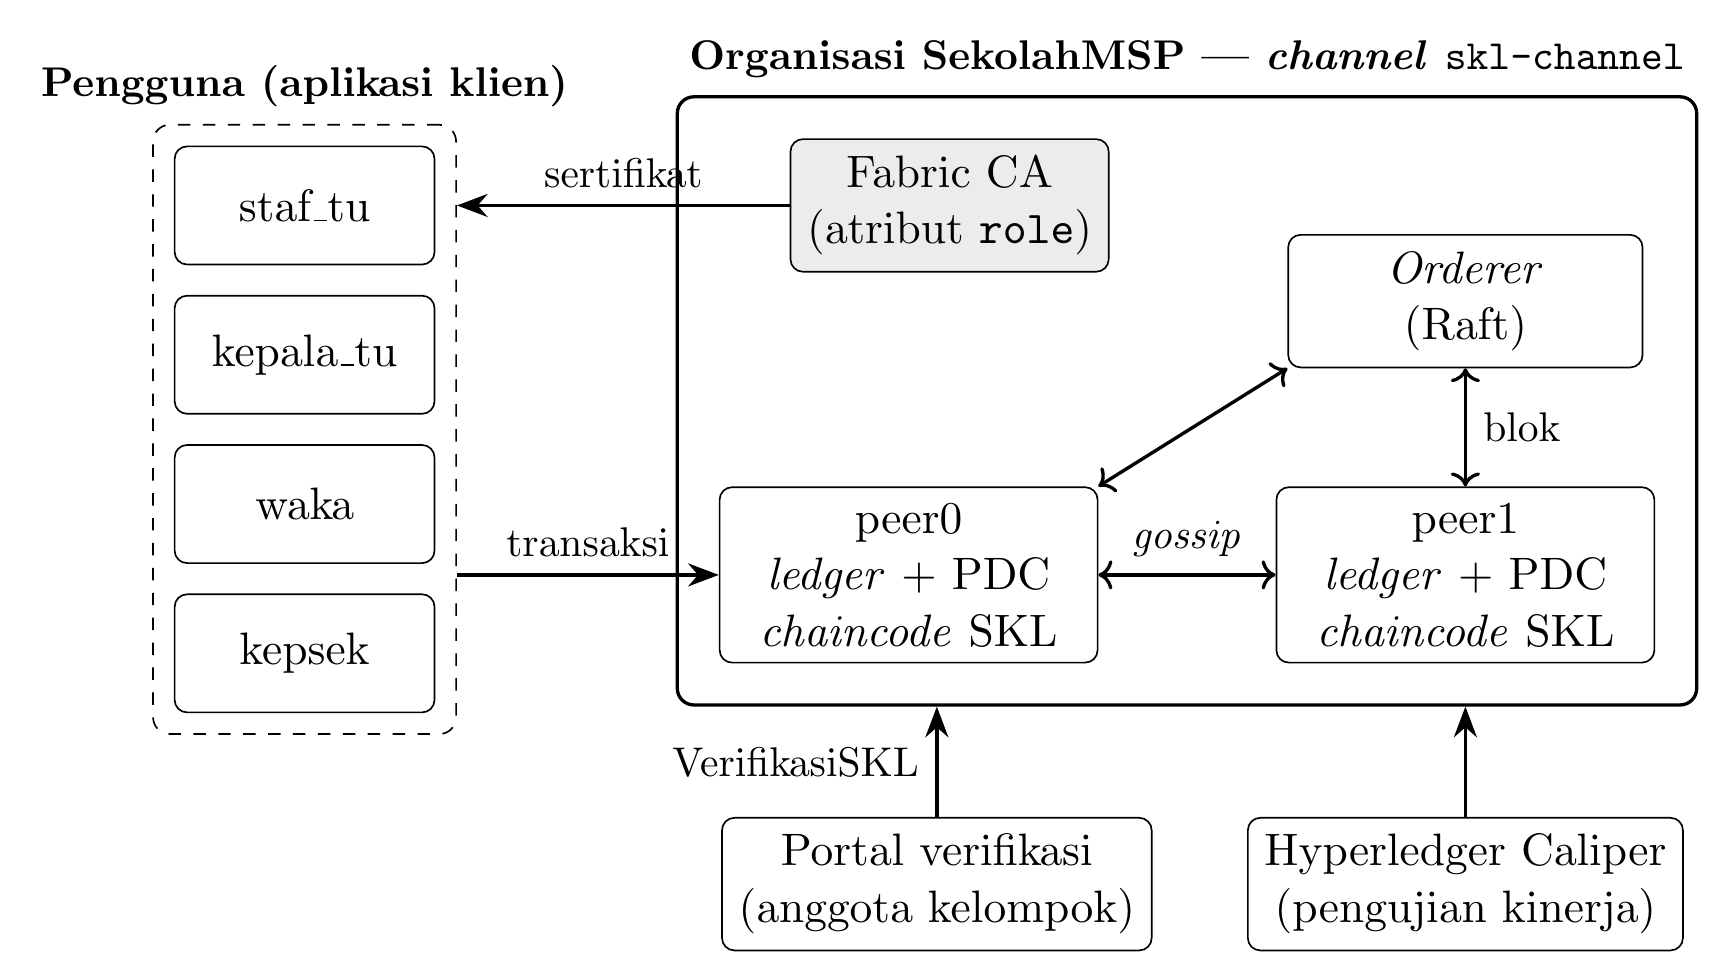
\includegraphics[width=0.95\textwidth]{figure/TopologiJaringanSKL.png}
    \caption{Rancangan topologi jaringan Hyperledger Fabric untuk SKL}
    \label{fig:topologi}
\end{figure}

Mesin status SKL ditunjukkan pada Gambar~\ref{fig:mesin_status}. Setiap SKL memiliki status DRAFT, DIVERIFIKASI, DISETUJUI\_WAKA, TERBIT, atau DICABUT, dan setiap fungsi hanya mengubah status apabila empat syarat terpenuhi: (1) atribut peran pemanggil sesuai fungsi; (2) status SKL saat ini sesuai urutan; (3) identitas pemanggil berbeda dari penginput dan belum pernah menyetujui SKL tersebut; serta (4) nilai \textit{hash} yang disetujui sama dengan nilai \textit{hash} yang tercatat. Penolakan oleh wakil kepala sekolah bidang kurikulum atau kepala sekolah mengembalikan status ke DRAFT disertai alasan, kepala tata usaha cukup tidak memverifikasi draf yang salah, dan perubahan data pada status DRAFT menghapus seluruh persetujuan sebelumnya.

\begin{figure}[H]
    \centering
    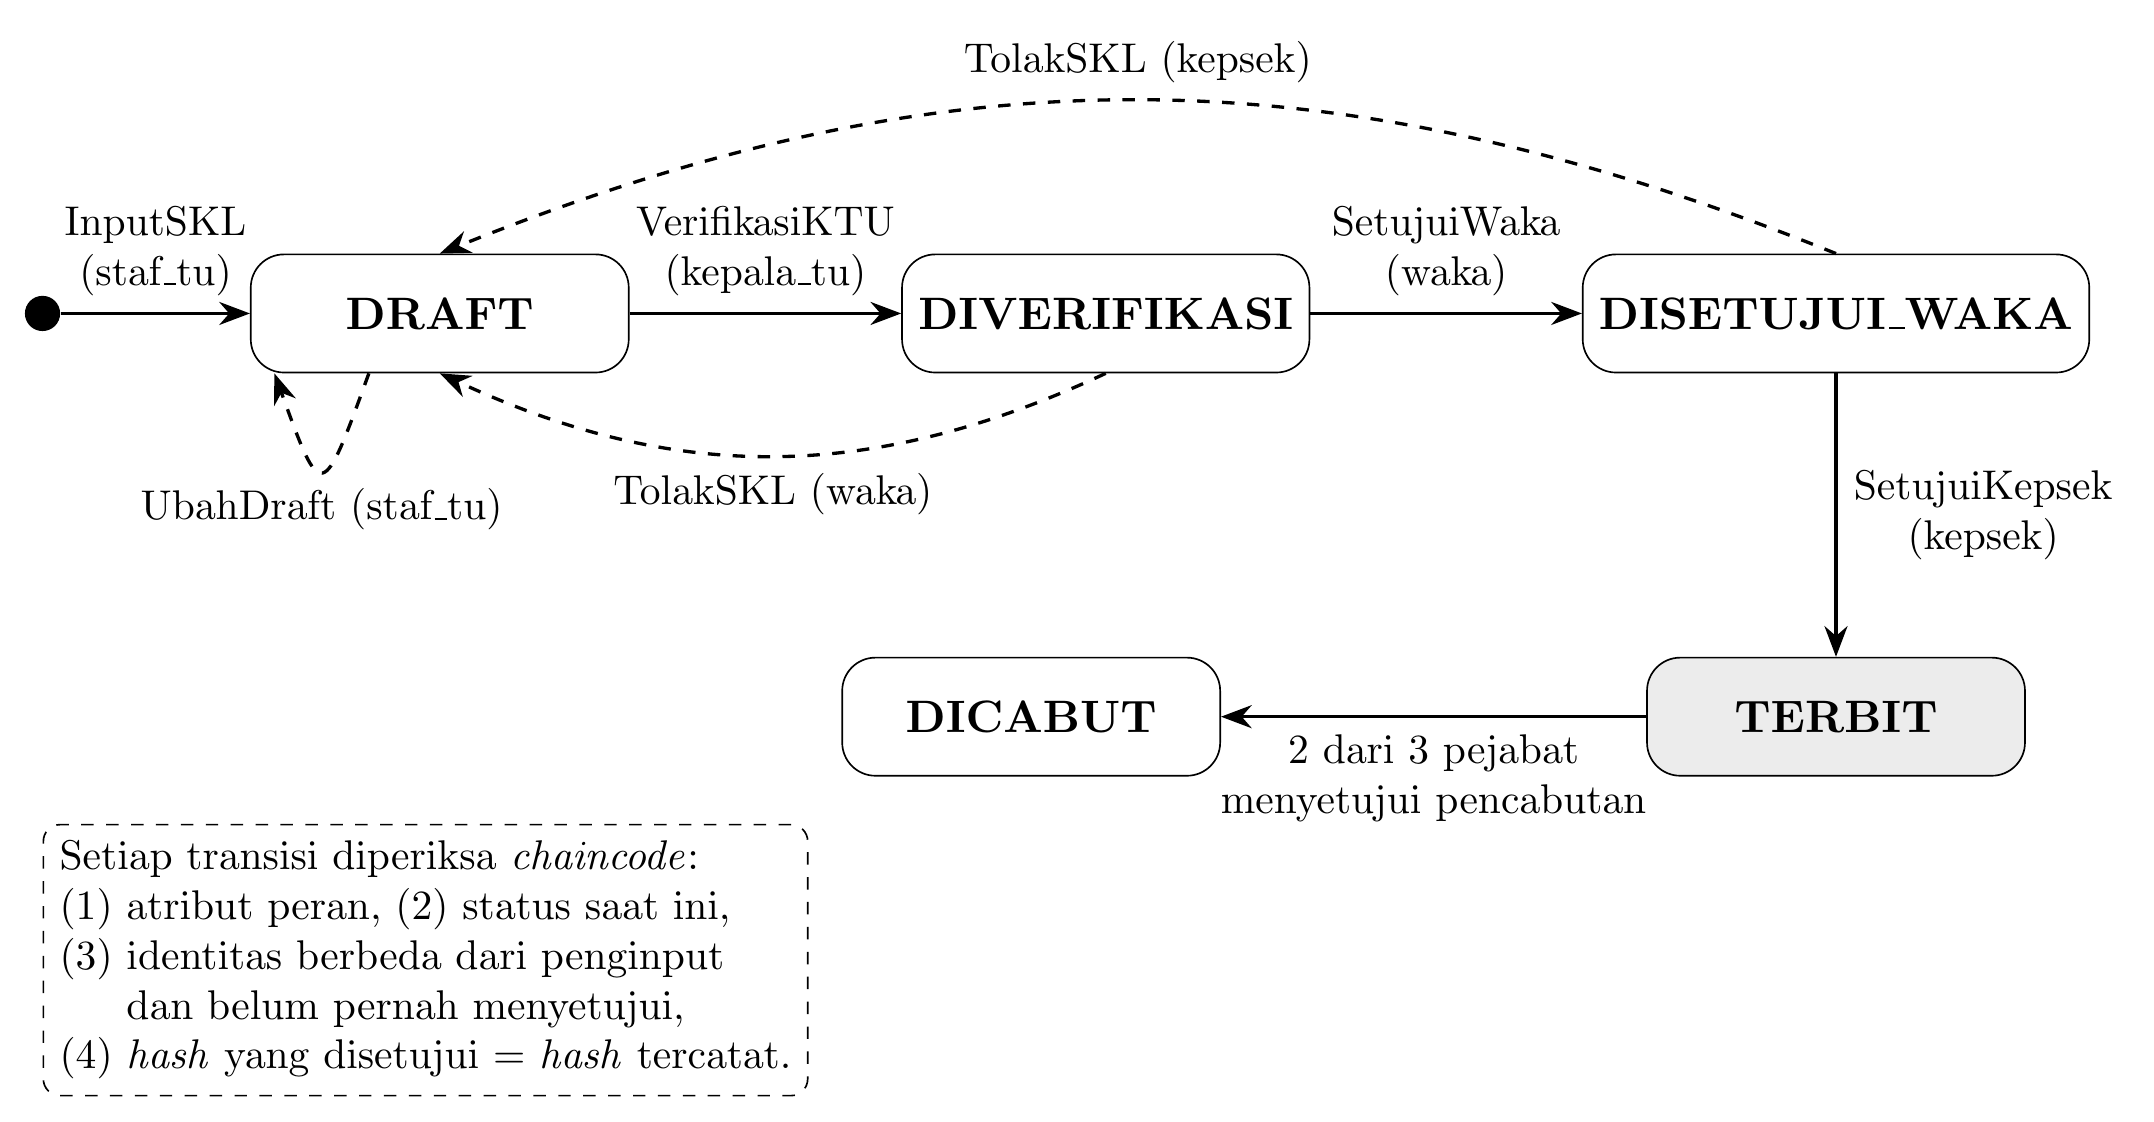
\includegraphics[width=0.85\textwidth]{figure/MesinStatusSKL.png}
    \caption{Mesin status penerbitan dan pencabutan SKL}
    \label{fig:mesin_status}
\end{figure}

Pembagian data antara \textit{ledger} dan \textit{private data collection} ditunjukkan pada Tabel~\ref{table:3.struktur}. Setiap SKL diberi ID SKL yang dibentuk dari tahun kelulusan dan NISN, misalnya \texttt{SKL-2026-0081234567}, sehingga setiap SKL dapat dikenali sejak masih berupa draf, sebelum nomor surat diberikan.

\begin{table}[H]
    \centering
    \caption{Rancangan struktur data SKL}
    \label{table:3.struktur}
    \footnotesize
    \renewcommand{\arraystretch}{1.25}
    \begin{tabular}{|>{\raggedright\arraybackslash}p{0.3\textwidth}|>{\raggedright\arraybackslash}p{0.3\textwidth}|>{\raggedright\arraybackslash}p{0.28\textwidth}|}
        \hline
        \textbf{Data} & \textbf{Lokasi penyimpanan} & \textbf{Dapat dibaca oleh} \\
        \hline
        ID SKL, nomor surat, nilai \textit{hash} $h_{SKL}$, status & \textit{Ledger} (\textit{world state}) & Anggota jaringan dan fungsi VerifikasiSKL \\
        \hline
        Riwayat persetujuan (identitas, peran, waktu, \textit{hash} yang disetujui) & \textit{Ledger} & Anggota jaringan \\
        \hline
        Format nomor surat dan penghitung nomor urut per tahun & \textit{Ledger} & Anggota jaringan \\
        \hline
        Daftar kode mata pelajaran yang berlaku & \textit{Ledger} (data acuan) & Anggota jaringan \\
        \hline
        Data lengkap SKL (identitas, daftar nilai per mata pelajaran, rata-rata) dan \textit{salt} & \textit{Private data collection} (collectionSKL) & Hanya anggota SekolahMSP \\
        \hline
    \end{tabular}
\end{table}

Data SKL setiap siswa disimpan sebagai satu dokumen JSON. Identitas siswa disimpan sebagai \textit{field} tetap, sedangkan nilai disimpan sebagai daftar pasangan kode mata pelajaran dan nilai, sehingga siswa dengan jumlah dan jenis mata pelajaran pilihan yang berbeda pada Kurikulum Merdeka tetap dapat disimpan dengan format yang sama. Kode mata pelajaran harus terdapat pada daftar kode yang berlaku, dan rata-rata nilai dihitung ulang oleh \textit{chaincode}; data ditolak apabila rata-rata yang diimpor tidak sama dengan hasil perhitungan. Untuk menghitung $h_{SKL}$, dokumen JSON disusun dalam bentuk baku (kanonik), yaitu \textit{field} diurutkan menurut nama, daftar nilai diurutkan menurut kode mata pelajaran, dan nilai ditulis sebagai teks dengan dua angka desimal, sehingga data yang sama selalu menghasilkan nilai \textit{hash} yang sama.

Data diimpor dari berkas leger nilai dalam format Excel/CSV, dengan satu baris untuk setiap siswa. Aplikasi mengubah setiap baris menjadi dokumen JSON dan mengirimkannya ke fungsi ImporSKL per kelas. Baris yang tidak lolos validasi dikembalikan kepada staf tata usaha untuk diperbaiki, sedangkan baris yang valid tersimpan sebagai draf. Selama berstatus DRAFT, data dapat diubah per siswa melalui fungsi UbahDraft atau dengan mengimpor ulang berkas yang telah diperbaiki; impor ulang hanya menimpa SKL yang masih berstatus DRAFT.

Nomor surat SKL dibuat otomatis dengan format yang ditetapkan sekolah, misalnya \texttt{421.3/\{urut\}/V.01/SMA/\{tahun\}}. Kepala tata usaha cukup menetapkan format dan nomor urut awal sekali melalui fungsi AturPenomoran, lalu nomor urut berikutnya dibuat oleh \textit{chaincode} secara berurutan tanpa nomor ganda. Nomor surat diberikan setelah SKL berstatus TERBIT, bukan saat input, agar SKL yang ditolak atau dicabut tidak meninggalkan nomor yang terlewat. Setelah kepala sekolah menyetujui, aplikasi otomatis memanggil fungsi BeriNomorSurat untuk seluruh SKL yang baru terbit dalam satu transaksi, dengan urutan per kelas lalu per abjad nama. Penomoran dilakukan dalam satu transaksi karena seluruh SKL memakai penghitung yang sama; apabila banyak transaksi mengubah penghitung tersebut secara bersamaan, hanya satu transaksi yang valid dan transaksi lainnya ditolak karena konflik versi data~\cite{FabricRWSet}. SKL baru dicetak, ditandatangani, dan distempel basah setelah memiliki nomor surat.

Data lengkap SKL disimpan pada koleksi data privat dengan konfigurasi seperti pada Tabel~\ref{table:3.pdc}. Data tidak dihapus otomatis karena masih diperlukan untuk penerbitan ulang dan pemeriksaan sekolah, tetapi dapat dihapus melalui fitur \textit{purge} apabila sekolah menetapkan masa retensi data~\cite{FabricPrivateData}.

\begin{table}[H]
    \centering
    \caption{Rancangan konfigurasi \textit{private data collection} SKL}
    \label{table:3.pdc}
    \footnotesize
    \renewcommand{\arraystretch}{1.25}
    \begin{tabular}{|>{\raggedright\arraybackslash}p{0.25\textwidth}|>{\raggedright\arraybackslash}p{0.25\textwidth}|>{\raggedright\arraybackslash}p{0.38\textwidth}|}
        \hline
        \textbf{Parameter} & \textbf{Nilai} & \textbf{Arti} \\
        \hline
        name & collectionSKL & Nama koleksi data privat SKL \\
        \hline
        policy & \texttt{OR('SekolahMSP.member')} & Hanya anggota SekolahMSP yang menyimpan data \\
        \hline
        requiredPeerCount & 1 & Minimal satu \textit{peer} lain menerima data sebelum transaksi disahkan \\
        \hline
        maxPeerCount & 1 & Jumlah maksimal \textit{peer} lain yang menerima data saat pengesahan \\
        \hline
        blockToLive & 0 & Data tidak dihapus otomatis \\
        \hline
        memberOnlyRead & true & Hanya anggota koleksi yang dapat membaca data \\
        \hline
        memberOnlyWrite & true & Hanya anggota koleksi yang dapat menulis data \\
        \hline
    \end{tabular}
\end{table}

\textit{Salt} berupa bilangan acak 128 bit yang berbeda untuk setiap SKL. Nilai ini dibangkitkan oleh aplikasi, bukan oleh \textit{chaincode}, karena \textit{chaincode} harus menghasilkan keluaran yang sama pada setiap \textit{peer} agar pengesahan cocok~\cite{FabricEndorsement}, sedangkan bilangan acak yang dibangkitkan di setiap \textit{peer} akan berbeda. \textit{Salt} disimpan bersama data SKL di \textit{private data collection} dan ikut dicantumkan pada \textit{QR code} SKL tercetak.

Pihak eksternal memverifikasi SKL tanpa mengakses data pribadi siswa yang tersimpan di jaringan, melalui tiga langkah yang ditunjukkan pada Gambar~\ref{fig:verifikasi_eksternal}. Pertama, verifikator memindai \textit{QR code} pada SKL yang diserahkan siswa; \textit{QR code} memuat ID SKL, nomor surat, data SKL dalam bentuk kanonik, dan \textit{salt}. Karena nilai disimpan sebagai kode mata pelajaran, ukuran data satu SKL kurang dari 1 KB sehingga masih dapat dimuat dalam satu \textit{QR code}. Kedua, portal verifikasi menghitung ulang $h' = \mbox{SHA-256}(D' \parallel s)$ dan memanggil fungsi VerifikasiSKL yang hanya membaca \textit{hash} dan status di \textit{ledger}, tanpa membaca \textit{private data collection}. Ketiga, portal menampilkan hasil VALID apabila $h'$ sama dengan $h_{SKL}$, nomor surat sama dengan yang tercatat, dan status SKL TERBIT; TIDAK COCOK apabila nilai \textit{hash} atau nomor surat berbeda; atau DICABUT apabila SKL telah dicabut. Setelah itu, verifikator mencocokkan data yang ditampilkan dengan data tercetak. Dengan cara ini, verifikator hanya melihat data yang memang sudah tercetak pada SKL yang diserahkan siswa, sedangkan pihak yang hanya melihat \textit{ledger} tidak dapat menebak isi SKL karena tidak memiliki \textit{salt}.

\begin{figure}[H]
    \centering
    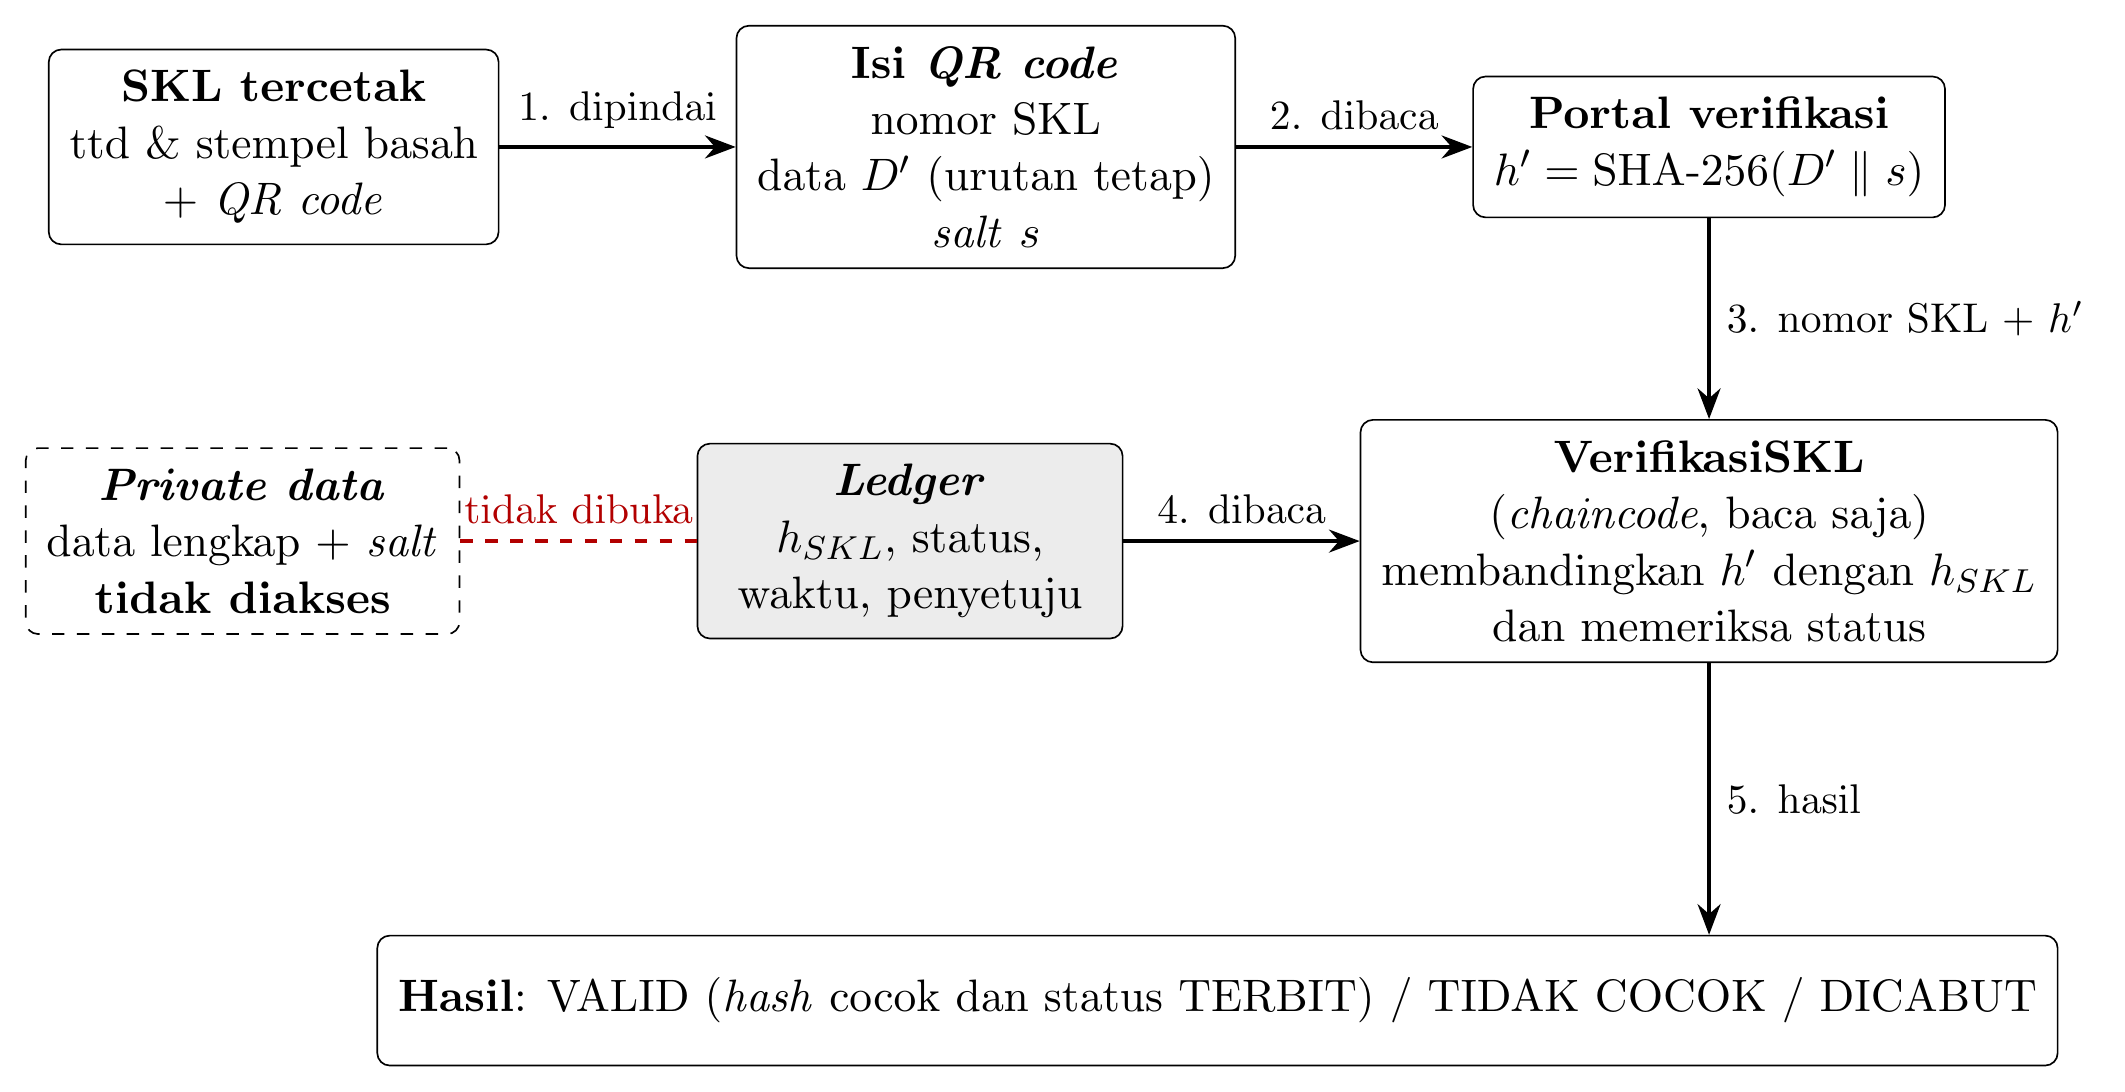
\includegraphics[width=0.85\textwidth]{figure/AlurVerifikasiEksternalSKL.png}
    \caption{Alur verifikasi SKL oleh pihak eksternal}
    \label{fig:verifikasi_eksternal}
\end{figure}

\textbf{4. \textit{Construction of Prototype}}

Peneliti membangun prototipe dengan langkah berikut: (1) menyiapkan Fabric CA dan mendaftarkan pengguna setiap peran beserta atribut \texttt{role} pada sertifikatnya; (2) membangun SekolahMSP, dua \textit{peer}, satu \textit{orderer}, dan \textit{channel} \texttt{skl-channel}; (3) menulis \textit{chaincode} dengan bahasa Go yang memuat impor massal, validasi data, mesin status, pemeriksaan atribut peran, pemisahan tugas, pengikatan \textit{hash}, dan penomoran surat; (4) mengonfigurasi \textit{private data collection} sesuai Tabel~\ref{table:3.pdc}; serta (5) memasang \textit{chaincode} dengan \textit{endorsement policy} dua \textit{peer}. Pengujian awal dilakukan setiap kali satu fungsi selesai dibuat.

\textbf{5. \textit{Deployment, Delivery}, dan \textit{Feedback}}

Prototipe didemonstrasikan kepada staf tata usaha, kepala tata usaha, dan wakil kepala sekolah bidang kurikulum dengan menjalankan alur impor berkas leger nilai, perbaikan draf, penerbitan, penomoran, penolakan, dan pencabutan SKL menggunakan data samaran. Umpan balik dicatat, dan apabila prototipe belum sesuai, peneliti kembali ke tahap \textit{communication} untuk iterasi berikutnya. Apabila sudah sesuai, prototipe dilanjutkan ke tahap pengujian.

\subsection{Metode Pengujian}
Pengujian dilakukan dengan tiga metode. Pertama, pengujian integritas data, yaitu mengubah isi SKL lalu memeriksa bahwa nilai \textit{hash}-nya tidak lagi cocok dengan yang tercatat di \textit{ledger}~\cite{Blanco2025Digital}. Kedua, \textit{black box testing} teknik \textit{state transition testing} untuk menguji kontrol akses dan alur persetujuan~\cite{Putri2024BlackBox,Augenio2025StateTransition}. Ketiga, pengujian kinerja dengan Hyperledger Caliper~\cite{Caliper}, termasuk perbandingan penerbitan oleh satu otoritas dan empat otoritas. Rancangan setiap pengujian dijelaskan pada Subbab~\ref{III.Pengujian}.

\section{Ilustrasi Perhitungan Metode}
Subbab ini memberikan contoh perhitungan menggunakan rumus pada Bab II. Data yang digunakan adalah data samaran, bukan data siswa sebenarnya, dan seluruh angka bersifat ilustrasi; nilai sebenarnya diperoleh pada Bab IV.

\subsection{Perhitungan Nilai \textit{Hash} SKL}
Contoh data SKL ditunjukkan pada Tabel~\ref{table:3.dataskl}. Untuk menyederhanakan contoh, daftar nilai hanya berisi tiga mata pelajaran.

\begin{table}[H]
    \centering
    \caption{Contoh data SKL (data samaran)}
    \label{table:3.dataskl}
    \footnotesize
    \renewcommand{\arraystretch}{1.25}
    \begin{tabular}{|>{\raggedright\arraybackslash}p{0.08\textwidth}|>{\raggedright\arraybackslash}p{0.35\textwidth}|>{\raggedright\arraybackslash}p{0.45\textwidth}|}
        \hline
        \textbf{No.} & \textbf{\textit{Field}} & \textbf{Nilai} \\
        \hline
        1 & ID SKL & SKL-2026-0081234567 \\
        \hline
        2 & NISN / NIS & 0081234567 / 12345 \\
        \hline
        3 & Nama & Andi Pratama \\
        \hline
        4 & Tempat dan tanggal lahir & Pringsewu, 12 Maret 2008 \\
        \hline
        5 & Nama orang tua & Budi Santoso \\
        \hline
        6 & Nilai & P03 (Ekonomi) = 91,37; U01 (Pendidikan Agama) = 90,80; U03 (Bahasa Indonesia) = 95,00 \\
        \hline
        7 & Rata-rata nilai (dihitung \textit{chaincode}) & $(91{,}37 + 90{,}80 + 95{,}00)/3 = 92{,}39$ \\
        \hline
        8 & Tanggal kelulusan & 2026-05-04 \\
        \hline
        9 & \textit{Salt} $s$ (128 bit) & \texttt{9f2c4e7a1b3d5f60\newline 718293a4b5c6d7e8} \\
        \hline
    \end{tabular}
\end{table}

\noindent Data tersebut disusun menjadi JSON kanonik $D_{SKL}$ sebagai berikut, lalu digabungkan dengan \textit{salt}.

\begin{center}
\scriptsize
\begin{tabular}{l}
\texttt{\{"id\_skl":"SKL-2026-0081234567","nama":"Andi Pratama",} \\
\texttt{"nama\_ortu":"Budi Santoso","nilai":[\{"kode":"P03",} \\
\texttt{"nilai":"91.37"\},\{"kode":"U01","nilai":"90.80"\},} \\
\texttt{\{"kode":"U03","nilai":"95.00"\}],"nis":"12345",} \\
\texttt{"nisn":"0081234567","rata\_rata":"92.39",} \\
\texttt{"tgl\_lulus":"2026-05-04","ttl":"Pringsewu, 12 Maret 2008"\}} \\
\end{tabular}
\end{center}

\noindent Nilai \textit{hash} dihitung dengan~\ref{eq:hash}, yaitu $h_{SKL} = \mbox{SHA-256}(D_{SKL} \parallel s)$. Hasil perhitungan untuk data asli dan dua contoh data yang diubah ditunjukkan pada Tabel~\ref{table:3.hash}.

\begin{table}[H]
    \centering
    \caption{Contoh perhitungan nilai \textit{hash} SKL}
    \label{table:3.hash}
    \footnotesize
    \renewcommand{\arraystretch}{1.25}
    \begin{tabular}{|>{\raggedright\arraybackslash}p{0.3\textwidth}|>{\raggedright\arraybackslash}p{0.58\textwidth}|}
        \hline
        \textbf{Data} & \textbf{Nilai \textit{hash} SHA-256 (heksadesimal)} \\
        \hline
        Data asli & \texttt{b0525c0bb70175d5a3abed0cd33e8016\newline 9689308630ac2af629805ca1d6518209} \\
        \hline
        Rata-rata nilai diubah dari 92.39 menjadi 99.39 & \texttt{acd7fecb8719a19fe606024a95697343\newline 896a3d589c6f63e168655a16e5fea92e} \\
        \hline
        Nama ditambah satu huruf (Andi Pratamaa) & \texttt{f3864cbd9401256203f5293a162d369f\newline f92909c9d94c039485d2b18ffe03514e} \\
        \hline
    \end{tabular}
\end{table}

Perubahan satu angka atau satu huruf menghasilkan nilai \textit{hash} yang sama sekali berbeda. Saat verifikasi, portal menghitung ulang $h'$ dari data dan \textit{salt} pada \textit{QR code}. Apabila $h'$ sama dengan $h_{SKL}$ di \textit{ledger}, hasilnya VALID; apabila berbeda, hasilnya TIDAK COCOK.

\subsection{Perhitungan Persentase Keberhasilan Pengujian}
Rancangan \textit{state transition testing} pada Tabel~\ref{table:3.st} terdiri atas 34 kasus uji. Misalkan 33 kasus uji memberikan hasil sesuai harapan, maka berdasarkan~\ref{eq:blackbox} diperoleh:

\begin{center}
$\begin{array}{rcl}
P & = & \displaystyle\frac{S_{sesuai}}{S_{total}} \times 100\% \\[12pt]
  & = & \displaystyle\frac{33}{34} \times 100\% \\[12pt]
  & = & 97{,}06\%
\end{array}$
\end{center}

\noindent Apabila seluruh 34 kasus uji sesuai harapan, maka $P = 100\%$.

\subsection{Perhitungan \textit{Throughput}, \textit{Latency}, dan \textit{Success Rate}}
Misalkan pada satu putaran Caliper dikirim 396 transaksi ImporSKL (satu SKL per transaksi) selama 16 detik, dengan 394 transaksi berhasil dan 2 transaksi gagal. Berdasarkan~\ref{eq:throughput}, \textit{throughput} dihitung sebagai berikut.

\begin{center}
$\begin{array}{rcl}
\mathit{Throughput} & = & \displaystyle\frac{\sum \mbox{transaksi berhasil}}{\mbox{total waktu pengujian}} \\[12pt]
  & = & \displaystyle\frac{394}{16} \\[12pt]
  & = & 24{,}63 \mbox{ TPS}
\end{array}$
\end{center}

\noindent Berdasarkan~\ref{eq:successrate}, \textit{success rate} dihitung sebagai berikut.

\begin{center}
$\begin{array}{rcl}
\mathit{Success\ rate} & = & \displaystyle\frac{Succ}{Succ + Fail} \times 100\% \\[12pt]
  & = & \displaystyle\frac{394}{394 + 2} \times 100\% \\[12pt]
  & = & 99{,}49\%
\end{array}$
\end{center}

\noindent Misalkan salah satu transaksi dikirim pada detik ke-3,20 dan tercatat pada detik ke-3,85. Berdasarkan~\ref{eq:latency}, \textit{latency} transaksi tersebut dihitung sebagai berikut.

\begin{center}
$\begin{array}{rcl}
\mathit{Latency} & = & t_{selesai} - t_{kirim} \\[6pt]
  & = & 3{,}85 - 3{,}20 \\[6pt]
  & = & 0{,}65 \mbox{ detik}
\end{array}$
\end{center}

\subsection{Perhitungan \textit{Overhead} Multi-Otoritas}
Misalkan rata-rata \textit{latency} empat transaksi pada skenario B ditunjukkan pada Tabel~\ref{table:3.latencyB}, sedangkan waktu penerbitan satu SKL pada skenario A adalah $\bar{L}_A = 0{,}60$ detik.

\begin{table}[H]
    \centering
    \caption{Contoh rata-rata \textit{latency} skenario B}
    \label{table:3.latencyB}
    \footnotesize
    \renewcommand{\arraystretch}{1.25}
    \begin{tabular}{|>{\raggedright\arraybackslash}p{0.08\textwidth}|>{\raggedright\arraybackslash}p{0.45\textwidth}|>{\raggedright\arraybackslash}p{0.3\textwidth}|}
        \hline
        \textbf{No.} & \textbf{Transaksi} & \textbf{\textit{Latency} (detik)} \\
        \hline
        1 & ImporSKL & 0,60 \\
        \hline
        2 & VerifikasiKTU & 0,55 \\
        \hline
        3 & SetujuiWaka & 0,58 \\
        \hline
        4 & SetujuiKepsek & 0,62 \\
        \hline
        \multicolumn{2}{|l|}{\textbf{Waktu penerbitan satu SKL ($\bar{L}_B$)}} & \textbf{2,35} \\
        \hline
    \end{tabular}
\end{table}

\noindent Berdasarkan~\ref{eq:overhead}, \textit{overhead} multi-otoritas dihitung sebagai berikut.

\begin{center}
$\begin{array}{rcl}
O & = & \displaystyle\frac{\bar{L}_B - \bar{L}_A}{\bar{L}_A} \times 100\% \\[12pt]
  & = & \displaystyle\frac{2{,}35 - 0{,}60}{0{,}60} \times 100\% \\[12pt]
  & = & 291{,}67\%
\end{array}$
\end{center}

\noindent Artinya, penerbitan oleh empat otoritas membutuhkan waktu sekitar 3,9 kali penerbitan oleh satu otoritas.

\section{Rancangan Pengujian} \label{III.Pengujian}
Pengujian dilakukan pada perangkat lunak, yaitu jaringan Hyperledger Fabric dan \textit{chaincode} SKL. Pengujian perangkat keras tidak dilakukan karena penelitian ini tidak membangun perangkat keras khusus. Pengujian dibagi menjadi pengujian fungsional (integritas data serta kontrol akses dan alur persetujuan) dan pengujian nonfungsional (kinerja jaringan).

\subsection{Pengujian Integritas Data}
Pengujian integritas data dilakukan dengan menerbitkan SKL, lalu memverifikasinya menggunakan data asli dan data yang telah diubah. Skenario pengujian ditunjukkan pada Tabel~\ref{table:3.integritas}.

\begin{table}[H]
    \centering
    \caption{Skenario pengujian integritas data}
    \label{table:3.integritas}
    \footnotesize
    \renewcommand{\arraystretch}{1.25}
    \begin{tabular}{|>{\raggedright\arraybackslash}p{0.1\textwidth}|>{\raggedright\arraybackslash}p{0.48\textwidth}|>{\raggedright\arraybackslash}p{0.3\textwidth}|}
        \hline
        \textbf{Kode} & \textbf{Skenario} & \textbf{Hasil yang diharapkan} \\
        \hline
        IT-01 & Verifikasi dengan data dan \textit{salt} asli & VALID \\
        \hline
        IT-02 & Rata-rata nilai diubah & TIDAK COCOK \\
        \hline
        IT-03 & Nama atau NISN diubah satu karakter & TIDAK COCOK \\
        \hline
        IT-04 & Data asli, tetapi \textit{salt} diubah & TIDAK COCOK \\
        \hline
        IT-05 & Nomor surat pada \textit{QR code} diubah & TIDAK COCOK \\
        \hline
        IT-06 & ID SKL tidak terdaftar di \textit{ledger} & TIDAK DITEMUKAN \\
        \hline
    \end{tabular}
\end{table}

\subsection{Pengujian Kontrol Akses dan Alur Persetujuan}
Pengujian ini menggunakan \textit{state transition testing}~\cite{Augenio2025StateTransition} terhadap mesin status pada Gambar~\ref{fig:mesin_status}. Setiap transisi yang sah diuji untuk memastikan diterima, sedangkan setiap transisi yang tidak sah diuji untuk memastikan ditolak. Kategori skenario uji ditunjukkan pada Tabel~\ref{table:3.skenario}.

\begin{table}[H]
    \centering
    \caption{Kategori skenario \textit{state transition testing}}
    \label{table:3.skenario}
    \footnotesize
    \renewcommand{\arraystretch}{1.25}
    \begin{tabular}{|>{\raggedright\arraybackslash}p{0.2\textwidth}|>{\raggedright\arraybackslash}p{0.42\textwidth}|>{\raggedright\arraybackslash}p{0.26\textwidth}|}
        \hline
        \textbf{Kategori} & \textbf{Contoh skenario} & \textbf{Hasil yang diharapkan} \\
        \hline
        Transisi sah & Setiap peran menjalankan fungsinya sesuai urutan (Tabel~\ref{table:3.fungsi}) & Diterima, status berpindah \\
        \hline
        Akses ilegal & Pengguna tanpa atribut peran, atau peran staf\_tu, memanggil SetujuiKepsek & Ditolak, status tetap \\
        \hline
        Manipulasi urutan persetujuan & waka menyetujui SKL berstatus DRAFT; kepsek menyetujui sebelum waka & Ditolak, status tetap \\
        \hline
        Transaksi berulang & Persetujuan yang sama dikirim dua kali; satu identitas menyetujui dua tahap & Transaksi kedua ditolak \\
        \hline
        Pemisahan tugas & Identitas penginput mencoba menyetujui SKL yang sama & Ditolak \\
        \hline
        Validasi impor dan penomoran & Baris berkas impor tidak valid; penomoran ulang SKL yang sudah bernomor & Baris ditolak; nomor tidak berubah \\
        \hline
        Perubahan setelah disetujui & Data diubah lalu persetujuan dikirim dengan \textit{hash} lama & Ditolak, status kembali DRAFT \\
        \hline
        Pencabutan tanpa kewenangan & staf\_tu mencabut SKL; hanya satu pejabat menyetujui pencabutan & Ditolak; status tetap TERBIT sampai dua pejabat menyetujui \\
        \hline
    \end{tabular}
\end{table}

Setiap kasus uji dijalankan dengan identitas peran tertentu terhadap SKL pada status tertentu, lalu keluaran dan status akhirnya dibandingkan dengan hasil yang diharapkan. Kasus uji yang disusun dari kategori tersebut ditunjukkan pada Tabel~\ref{table:3.st}.

\begingroup
\setlength{\tabcolsep}{3pt}
\renewcommand{\arraystretch}{1.2}
\footnotesize
\begin{longtable}{|>{\raggedright\arraybackslash}p{0.09\textwidth}|>{\raggedright\arraybackslash}p{0.17\textwidth}|>{\raggedright\arraybackslash}p{0.36\textwidth}|>{\raggedright\arraybackslash}p{0.26\textwidth}|}
    \caption{Rancangan kasus uji \textit{state transition testing}}
    \label{table:3.st}\\
    \hline
    \textbf{Kode} & \textbf{Kategori} & \textbf{Kasus uji} & \textbf{Hasil yang diharapkan} \\
    \hline
    \endfirsthead
    \hline
    \textbf{Kode} & \textbf{Kategori} & \textbf{Kasus uji} & \textbf{Hasil yang diharapkan} \\
    \hline
    \endhead
    ST-01 & Transisi sah & staf\_tu memanggil ImporSKL dengan berkas 36 siswa yang seluruhnya valid & Diterima, 36 SKL berstatus DRAFT \\ \hline
    ST-02 & Transisi sah & staf\_tu memanggil UbahDraft pada SKL berstatus DRAFT & Diterima, \textit{hash} baru, persetujuan sebelumnya dihapus \\ \hline
    ST-03 & Transisi sah & kepala\_tu memanggil VerifikasiKTU untuk satu kelas berstatus DRAFT & Diterima, seluruh SKL berstatus DIVERIFIKASI \\ \hline
    ST-04 & Transisi sah & waka memanggil SetujuiWaka pada SKL berstatus DIVERIFIKASI & Diterima, status DISETUJUI\_\allowbreak WAKA \\ \hline
    ST-05 & Transisi sah & kepsek memanggil SetujuiKepsek pada SKL berstatus DISETUJUI\_\allowbreak WAKA & Diterima, status TERBIT \\ \hline
    ST-06 & Transisi sah & kepala\_tu memanggil AturPenomoran dengan nomor awal 191 tahun 2026 & Diterima, format dan nomor awal tersimpan \\ \hline
    ST-07 & Transisi sah & BeriNomorSurat dipanggil untuk tiga SKL berstatus TERBIT & Nomor 191, 192, dan 193 diberikan berurutan \\ \hline
    ST-08 & Transisi sah & waka memanggil TolakSKL pada SKL berstatus DIVERIFIKASI & Diterima, status DRAFT \\ \hline
    ST-09 & Transisi sah & kepsek memanggil TolakSKL pada SKL berstatus DISETUJUI\_\allowbreak WAKA & Diterima, status DRAFT \\ \hline
    ST-10 & Transisi sah & Dua pejabat berbeda memanggil SetujuiPencabutan pada SKL berstatus TERBIT & Diterima, status DICABUT \\ \hline
    ST-11 & Transisi sah & Verifikator memanggil VerifikasiSKL dengan \textit{hash} dan nomor surat yang cocok & VALID, status tidak berubah \\ \hline
    ST-12 & Validasi data & ImporSKL dengan satu baris ber-NISN sembilan digit & Baris tersebut ditolak, baris lain berstatus DRAFT \\ \hline
    ST-13 & Validasi data & ImporSKL dengan nilai 101 & Baris tersebut ditolak \\ \hline
    ST-14 & Validasi data & ImporSKL dengan rata-rata yang tidak sesuai perhitungan & Baris tersebut ditolak \\ \hline
    ST-15 & Validasi data & ImporSKL dengan kode mata pelajaran yang tidak terdaftar & Baris tersebut ditolak \\ \hline
    ST-16 & Validasi data & ImporSKL dengan NISN yang sudah memiliki SKL bukan DRAFT & Baris tersebut ditolak \\ \hline
    ST-17 & Akses ilegal & Identitas tanpa atribut \texttt{role} memanggil ImporSKL & Ditolak \\ \hline
    ST-18 & Akses ilegal & staf\_tu memanggil SetujuiKepsek & Ditolak, status tetap \\ \hline
    ST-19 & Akses ilegal & Identitas dengan sertifikat dari CA yang tidak dipercaya SekolahMSP mengirim transaksi & Ditolak oleh jaringan \\ \hline
    ST-20 & Akses ilegal & staf\_tu memanggil AturPenomoran & Ditolak \\ \hline
    ST-21 & Manipulasi urutan & waka memanggil SetujuiWaka pada SKL berstatus DRAFT & Ditolak, status tetap \\ \hline
    ST-22 & Manipulasi urutan & kepsek memanggil SetujuiKepsek pada SKL berstatus DIVERIFIKASI & Ditolak, status tetap \\ \hline
    ST-23 & Manipulasi urutan & staf\_tu memanggil UbahDraft pada SKL berstatus DIVERIFIKASI & Ditolak, status tetap \\ \hline
    ST-24 & Manipulasi urutan & kepala\_tu memanggil VerifikasiKTU untuk lima SKL, salah satunya berstatus TERBIT & Empat SKL berpindah status, satu SKL dilaporkan gagal \\ \hline
    ST-25 & Manipulasi urutan & BeriNomorSurat dipanggil untuk SKL berstatus DISETUJUI\_\allowbreak WAKA & Tidak diberi nomor \\ \hline
    ST-26 & Transaksi berulang & waka mengirim SetujuiWaka dua kali untuk SKL yang sama & Transaksi kedua ditolak \\ \hline
    ST-27 & Transaksi berulang & BeriNomorSurat dipanggil dua kali untuk SKL yang sama & Nomor surat tidak berubah \\ \hline
    ST-28 & Transaksi berulang & Pejabat yang sama mengirim SetujuiPencabutan dua kali & Status tetap TERBIT \\ \hline
    ST-29 & Pemisahan tugas & Identitas penginput (diberi atribut kepala\_tu untuk pengujian) memanggil VerifikasiKTU atas SKL yang diimpornya & Ditolak \\ \hline
    ST-30 & Ikatan \textit{hash} & waka memanggil SetujuiWaka dengan \textit{hash} lama setelah data diubah & Ditolak \\ \hline
    ST-31 & Pencabutan tanpa kewenangan & staf\_tu memanggil SetujuiPencabutan & Ditolak \\ \hline
    ST-32 & Pencabutan tanpa kewenangan & Hanya satu pejabat memanggil SetujuiPencabutan & Status tetap TERBIT \\ \hline
    ST-33 & Verifikasi & VerifikasiSKL dengan \textit{hash} dari data yang diubah & TIDAK COCOK \\ \hline
    ST-34 & Verifikasi & VerifikasiSKL pada SKL berstatus DICABUT & DICABUT \\ \hline
\end{longtable}
\endgroup

\subsection{Pengujian Kinerja}
Pengujian kinerja dilakukan dengan Hyperledger Caliper pada jaringan yang berjalan di satu laptop sesuai Subbab~3.3.1. Beban setiap putaran adalah 396 transaksi, sesuai jumlah siswa per angkatan, dan dikirim dengan tiga laju pengiriman tetap, yaitu 10, 25, dan 50 TPS. Setiap kombinasi dijalankan tiga kali dan diambil rata-ratanya. Untuk mengetahui \textit{overhead} multi-otoritas, digunakan dua skenario dengan beban yang sama. Skenario A adalah penerbitan oleh satu otoritas, yaitu satu transaksi per SKL yang langsung menghasilkan status TERBIT, menggunakan \textit{chaincode} terpisah khusus pengujian sehingga aturan multi-otoritas pada \textit{chaincode} utama tidak dilemahkan. Skenario B adalah penerbitan oleh empat otoritas, yaitu empat transaksi berurutan per SKL sesuai Tabel~\ref{table:3.fungsi}, masing-masing berisi satu SKL agar sebanding dengan skenario A. Selain itu, dua putaran tambahan mengukur efisiensi rancangan, yaitu impor massal per kelas dan penomoran surat untuk seluruh angkatan dalam satu transaksi. Penomoran tidak diuji dengan laju kirim tinggi karena memakai penghitung bersama yang memang dirancang untuk dijalankan dalam satu transaksi~\cite{FabricRWSet}. Rancangan putaran pengujian ditunjukkan pada Tabel~\ref{table:3.caliper}.

\begin{table}[H]
    \centering
    \caption{Rancangan putaran pengujian Caliper}
    \label{table:3.caliper}
    \footnotesize
    \renewcommand{\arraystretch}{1.25}
    \begin{tabular}{|>{\raggedright\arraybackslash}p{0.13\textwidth}|>{\raggedright\arraybackslash}p{0.38\textwidth}|>{\raggedright\arraybackslash}p{0.16\textwidth}|>{\raggedright\arraybackslash}p{0.2\textwidth}|}
        \hline
        \textbf{Skenario} & \textbf{Fungsi yang diuji} & \textbf{Transaksi per putaran} & \textbf{Laju kirim (TPS)} \\
        \hline
        A & TerbitkanLangsung (satu otoritas, satu SKL per transaksi) & 396 & 10, 25, 50 \\
        \hline
        B & ImporSKL, VerifikasiKTU, SetujuiWaka, SetujuiKepsek (berurutan, satu SKL per transaksi) & 396 per fungsi & 10, 25, 50 \\
        \hline
        Impor massal & ImporSKL (36 SKL per transaksi) & 11 & Dikirim berurutan \\
        \hline
        Penomoran & BeriNomorSurat (396 SKL dalam satu transaksi) & 1 & -- \\
        \hline
        Kueri & VerifikasiSKL & 396 & 10, 25, 50 \\
        \hline
    \end{tabular}
\end{table}

Metrik yang diukur adalah \textit{throughput}, \textit{latency}, dan \textit{success rate} untuk setiap fungsi, \textit{overhead} multi-otoritas dari perbandingan skenario A dan B, serta total waktu impor massal dan penomoran untuk satu angkatan.

\subsection{Hipotesis}
Hipotesis hasil yang diharapkan dari penelitian ini adalah sebagai berikut.
\begin{enumerate}
    \item Seluruh perubahan isi SKL pada pengujian integritas terdeteksi, yaitu hasil verifikasi menjadi TIDAK COCOK.
    \item Seluruh kasus uji \textit{state transition testing} memberikan hasil sesuai harapan, sehingga persentase keberhasilan pengujian mencapai 100\%.
    \item \textit{Success rate} transaksi pada seluruh putaran Caliper mendekati 100\%, dan \textit{latency} setiap transaksi berada di bawah satu detik pada laju kirim rendah, sebanding dengan hasil Dash dkk.~\cite{Dash2025Hyperledger}.
    \item Impor massal 396 SKL yang dikirim per kelas dan penomoran 396 SKL dalam satu transaksi berhasil seluruhnya, dengan nomor surat berurutan tanpa nomor ganda maupun nomor yang terlewat.
    \item Waktu penerbitan satu SKL pada skenario B sekitar empat kali skenario A karena memerlukan empat transaksi berurutan, sehingga \textit{overhead} multi-otoritas sekitar 300\%. \textit{Overhead} ini dianggap dapat diterima apabila waktu pencatatan 396 SKL di jaringan tetap jauh lebih singkat daripada waktu penyusunan SKL saat ini yang memerlukan beberapa hari kerja.
\end{enumerate}